\chapter{Fundamentos te\'oricos}\label{capit:cap2}
\vspace{-2.0325ex}%
\noindent
\rule{\textwidth}{0.5pt}
\vspace{-5.5ex}% 
\newcommand{\pushline}{\Indp}% Indent puede ir o no :p

\section{Introducci\'on}\label{secc:introduccion}
La ansiedad es un fen\'omeno con el que nuestra sociedad se encuentra \'intimamente relacionada. Todos la sentimos multiples veces a lo largo de nuestras vidas, al dar un discurso en p\'ublico, al ser entrevistado para un nuevo trabajo o durante un examen. Es parte de lo que nos mantiene alertas y listos para enfrentar las situaciones de d\'ia a d\'ia. Sin embargo, solemos no darle la importancia que significa para las personas que sufren de elevados niveles de ansiedad y de los beneficios que la tecnolog\'ia puede brindarles. En este cap\'itulo, se define la ansiedad, la manera en que se origina, como afecta a los cuidadores y como podemos medirla.



\section{Qu\'e es la Ansiedad?}\label{secc:ansiedad}

La ansiedad es una emoci\'on caracterizada por sensaciones de tensi\'on, pensamientos de preocupaci\'on y cambios f\'isicos como incremento en la presi\'on arterial \citep{psychologyapa}, aumento de la sudoraci\'on y palpitaciones, entre otras respuestas fisiol\'ogicas. Estas manifestaciones se dan en determinados lapsos de tiempos durante la vida del individuo. Durante estos lapsos, se dice que el sujeto se encuentra en un estado mental de ansiedad [ref].

Este estado mental es \'util para los humanos, debido a que la ansiedad es una reacci\'on normal del cuerpo para lograr objetivos, o lograr sobrevivir ante a una amenaza. Sin embargo, cuando la persona experimenta un nivel de ansiedad el cual es tan alto que no le permite manejar su vida normal, se dice que la persona tiene un desorden de ansiedad\citep{repetto2013}. 

\subsection{Ansiedad y estr\'es}\label{secc:anxietyandstress}
Si bien, en ocasiones el estr\'es y la ansiedad son conceptos que se usan de manera intercambiable, existen diferencias entre ambos. El estr\'es es definido como el desvalance entre la carga mental dada y la percepci\'on de las habilidades que el individuo tiene para lidiar con dicha carga[ref]. Este desvalance puede hacer que la ansiedad aumente, mientras que la ansiedad puede a su vez generar estr\'es. La relaci\'on entre el estr\'es y la ansiedad es la ansiedad es la se\~nal psicofisiol\'ogica de que la respuesta al estr\'es ha sido iniciada \citep{PMID2235645}.


\subsection{``State Anxiety'' y ``Trait Anxiety''}\label{secc:anxieystatevstrait}
Existen dos clasificaciones de ansiedad reconocidas por la \textit{American Psychological Association} \citep{psychologyapa} , ``State Anxiety'' y ``Trait Anxiety''. Las cuales se mencionan a continuaci\'on.

\begin{itemize}
	\item{\textbf{State Anxiety:}} Es una manifestaci\'on de ansiedad a cerca de un evento \textbf{presente} bien definido. Normalmente la persona se encuentra conciente de la fuente de su ansiead. 
	\item{\textbf{Trait Anxiety:}} Es una manifestaci\'on a largo plazo de la ansiedad, en la que el individuo puede entrar al estado ansioso sin saber la raz\'on concreta. Las personas con personalidades t\'imidas tienden a sufrir mas de este tipo de ansiedad. [ref]

\end{itemize}

A pesar de que los efectos negativos en la calidad de vida de las personas que sufren de ``Trait Anxiety'' son mas fuertes, este trabajo est\'a enfocado en ``State Anxiety'' debido a que es mas f\'acil de cuantificar y medir por medio de sensores.

\section{Demencia}\label{secc:dementia}
La demencia es un s\'indrome del declive de las habilidades cognitivas. Los s\'intomas comunes son: problemas de memoria, dificultades para realizar tareas familiares, mal juicio, deterioro del lenguaje hablado y cambios de humor\citep{Aziz}. Afecta alrededor de el 4\% de las personas mayores de 65 a\~nos y al 40\% de las personas mayores de 90. La demencia suele manifestarse en s\'indromes como el de Alzheimer. Las personas con demencia necesitan de una persona que cuide de ellos, normalmente durante el resto de su vida. Usualmente necesitan ayuda en las actividades de la vida diaria (Activities of Daily Life), siendo esto una carga para los cuidadores.

\section{Cuidadores}\label{secc:caregivers}
Uno de los sectores de poblaci\'on vulnerables, es el de los cuidadores de personas con demencia. Se encuentra documentado que los cuidadores, al llevar una carga f\'isica, cognitiva y emocional derivada de su labor les genera padecimientos como ansiedad, estr\'es, y hasta la muerte\citep{Chen2013}. Debido a que los cuidadores no necesariamente son personas con una formaci\'on profesional, estos efectos pueden verse aumentados. Por lo general, los cuidadores que son familiares del paciente son a\'un m\'as afectados ya que necesitan administrar el tiempo de trabajo, familia, actividades sociales y la actividad misma del cuidado del paciente.
			%Cuales son las situaciones ( escenarios ) en los que los CUIDADORES presentan ansiedad?

\subsection{C\'omo se genera la ansiedad en los cuidadores?}\label{secc:caregiverburden}

\begin{figure}[h]
	\centering
	\subfigure[]{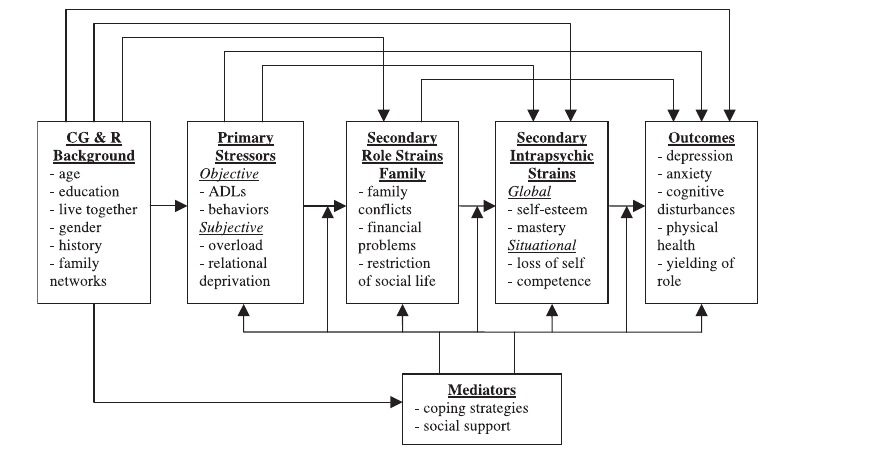
\includegraphics[width=160mm,height=80mm]{./Figures/img_frame}} 
	\caption{El modelo de ansiedad en cuidadores (Pearlin et. al 1990)} \label{fig:modeloAnsiedad}
\end{figure}
El modelo de la ansiedad en cuidadores, es definido por Pearlin como un conjunto de caracter\'isticas del individuo, factores de estres, carga del cuidador y estrategias de afrontamiento, las cuales tienen como salida efectos positivos o negativos\citep{Pearlin01101990}. A continuaci\'on, se explica el modelo de Pearlin elemento por elemento.
	\subsection{Caracter\'isticas del individuo}{\label{secc:modeloAnsiedadCaregivers}}
		La edad y sexo, el nivel de educaci\'on y los lazos que tiene el cuidador con la persona con demencia son los principales factores que pueden hacer mas suceptible a los cuidadores de sufrir los efectos de la ansiedad. Un adolescente sin experiencia de cuidador podr\'ia sentirse en grandes aprietos al tratar de satisfacer una necesidad de una persona con demencia. De la misma forma, es dif\'icil emocionalmente para los cuidadores ver como el declive cognitivo de un familiar con demencia se va desarrollando hasta el grado de que no reconozca a sus propios hijos.
	\subsection{Factores de estr\'es primarios}{\label{secc:modeloAnsiedadStressFactors}}
		Los factores de estr\'es, o la carga f\'isica y/o cognitiva se dividen en dos: Los factores de estr\'es objetivos y los subjetivos. Los objetivos son aquellos que podemos medir como las actividades de la vida diaria (ADL) y los comportamientos. Estos los podemos medir como la frecuencia y severidad de los eventos en un espacio de tiempo y podemos hacer un registro de ellos. Por otra parte, los subjetivos son aquellos que afectan a la percepci\'on del cuidador, como la sobrecarga y la deprivaci\'on relacional.
	\subsection{Carga del cuidador}{\label{secc:modeloAnsiedadSecondaryroles}}
		Comunmente, los cuidadores son familiares que viven en la misma casa que la persona con demencia, por lo que suelen tener diferentes roles sociales. Muchos de ellos son madres, padres o hijos que tienen la obligaci\'on de trabajar y proveer de recursos al hogar. La carga extra de cuidar a alguien puede resultar en un desequilibrio emocional del cuidador.
	
	\subsection{Estrategias de afrontamiento}{\label{secc:modeloAnsiedadCoping}}
	Algunos cuidadores logran reducir su nivel de ansiedad por medio de estrategias de afrontamiento. Ejercicios de respiraci\'on, la b\'usqueda de apoyo de familiares y amigos o el consuelo religioso \citep{Sharma20121287} son algunas de las t\'ecnicas que mas sirven a los cuidadores. Sin embargo, no todos ellos las utilizan o utilizan estrategias negativas como el uso de alcohol o drogas.

	La salida de este modelo, afecta en los niveles de depresi\'on, ansiedad y salud f\'isica del cuidador. El buen uso de las estrategias de afrontamiento, el balance de roles y carga del cuidador pueden ayudar a reducir su ansiedad y mejorar su salud f\'isica y/o mental.

	\subsection{Cuidadores Formales e Informales}\label{secc:caregivers}


	\subsection{Se\~nales fisiol\'ogicas relacionadas}\label{secc:signals}
	El Sistema Aut\'onomo Central (SAC) es una divisi\'on del Sistema Nervioso Perif\'erico (SNP) el cual controla el funcionamiento de los \'organos viscerales. Controla las funciones del cuerpo como la respiraci\'on, digesti\'on, ritmo cardi\'aco, y deseo sexual de manera inconsciente. Est\'a dividido por dos subsistemas: el \textit{Sistema Nervioso Simp\'atico} y el \textit{Sistema Nervioso Parasimp\'atico} (Ver Figura ~\ref{fig:modeloSNP}). Ambos controlan las mismas funciones, pero de manera an\'aloga. Mientras el SNS aumenta los latidos del coraz\'on, el SNP lo disminuye.

\begin{figure}[h]
	\centering
	\subfigure[]{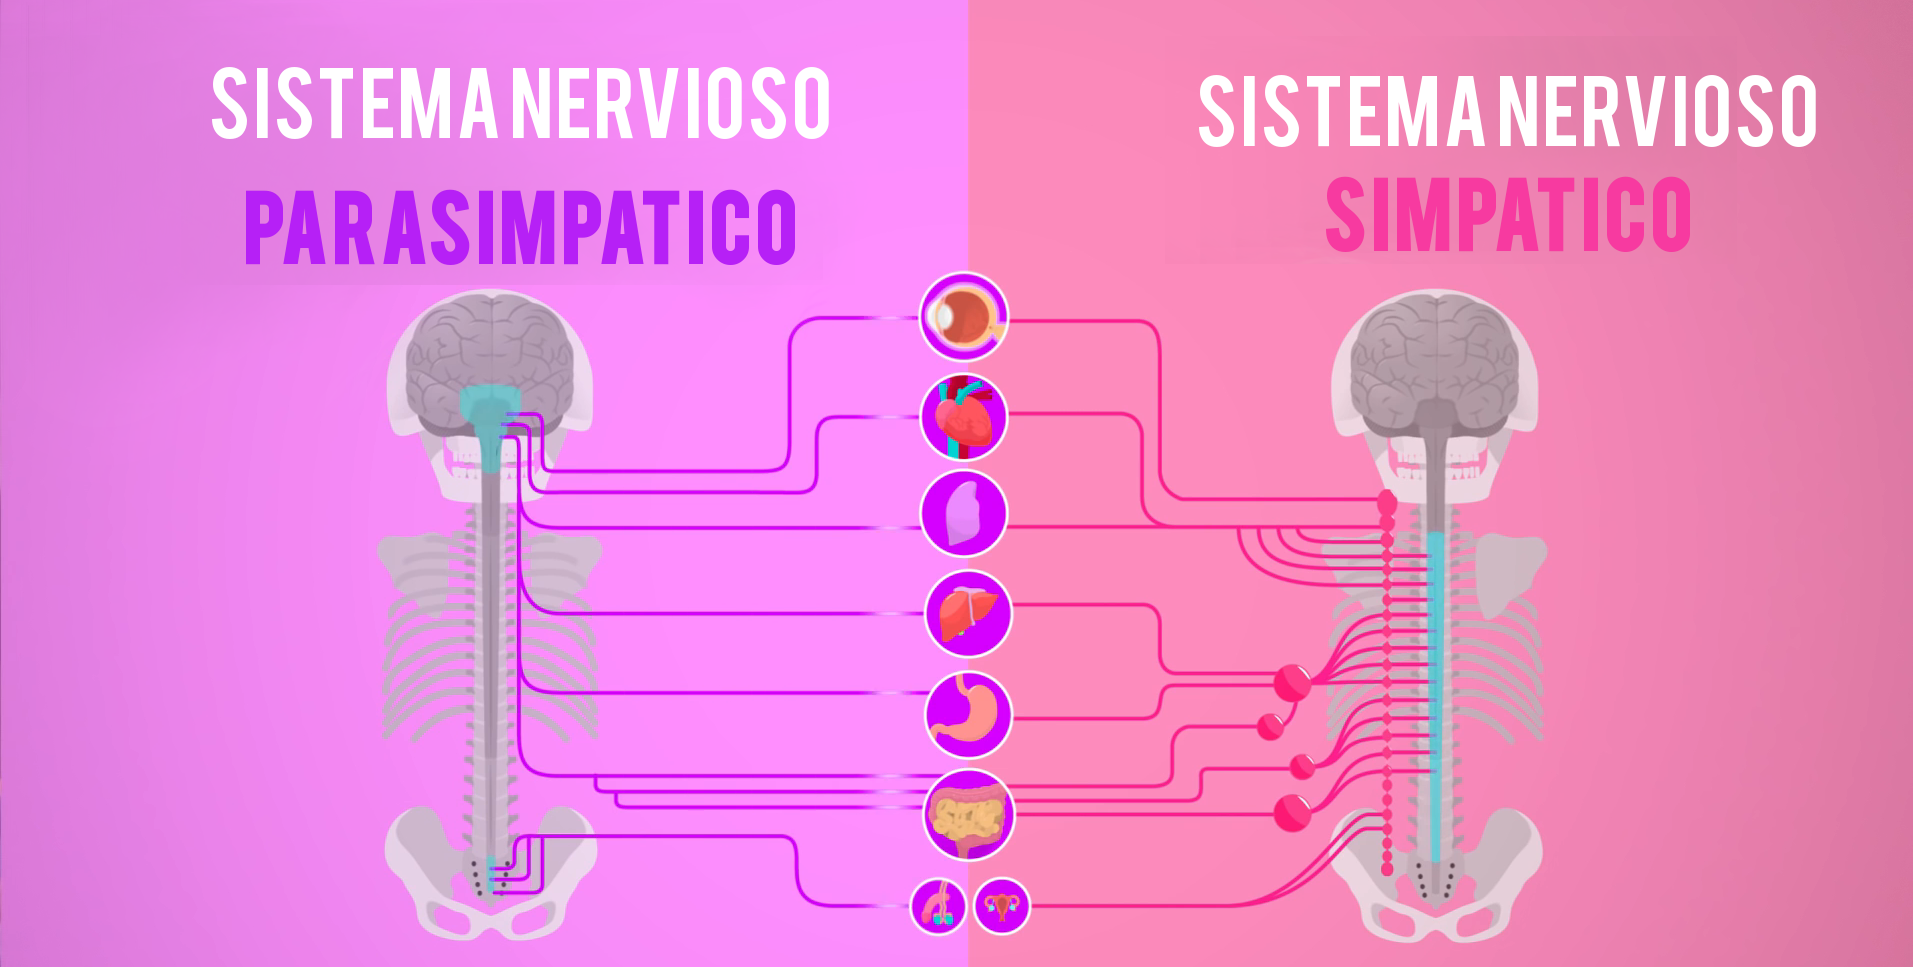
\includegraphics[width=160mm,height=80mm]{./Figures/img_snc}} 
	\caption{El sistema Aut\'onomo central (Crash Course A\&P \#13) \label{fig:modeloSNP}}
\end{figure}

Los efectos de la ansiedad se manifestan en el ritmo card\'iaco [ref], respiraci\'on [ref] y sudoraci\'on [ref] los cuales son controlados por el SAC. Normalmente, el individuo no tiene control sobre los cambios en sus funciones corporales. Algunos de estos cambios, como la sudoraci\'on y el ritmo card\'iaco pueden ser cuantificados por medio de sensores. A continuaci\'on, se explican algunas se\~nales de estos cambios usadas para detectar la ansiedad.

	\subsubsection{Respuesta Galv\'anica de la Piel (GSR)}\label{secc:gsr}
	Uno de los efectos que la ansiedad causa sobre el cuerpo es la sudoraci\'on. El sudor est\'a formado mayormente por agua y minerales y ayuda a mantener la temperatura corporal. Un efecto secundario de la presencia del sudor es el cambio en la conductancia el\'ectrica de la piel, siendo esta definida como \textit{``la facilidad que ofrece un material al paso de la corrente el\'ectrica''}. Esta capacidad de conductividad es denotada por la unidad del sistema internacional \textit{Siemen ($S$)}. La unidad $S$ est\'a definida por: $S = \Omega^{-1} = \dfrac{A}{V}$. Donde $\Omega$ es el ohm, $A$ es el ampero y $V$ es el Voltio. Debido a que los valores de las mediciones son comunmente muy peque\~nas, las mediciones son denotadas por el prefijo $\mu$.
	\begin{figure}[h]
		\centering
		\subfigure[]{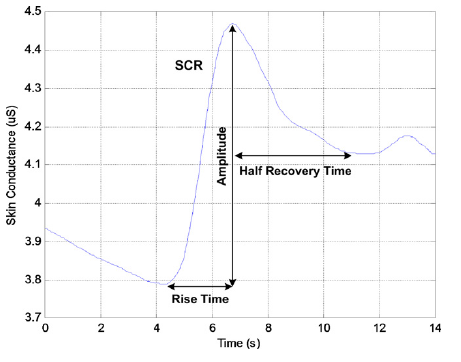
\includegraphics[width=100mm,height=80mm]{./Figures/img_gsr}} 
		\caption{Se\~nal t\'ipica de GSR \label{fig:GSRsignal}}
	\end{figure}

	La se\~nal de GSR se encuentra compuesta por dos partes: Un componente base y un componente t\'onico \citep{Katsis2011261}. El componente base corresponde a un nivel promedio sin un \textit{stimuli} en concreto, mientras que el componente t\'onico es la reacci\'on a un est\'imulo. La figura ~\ref{fig:GSRsignal} ejemplifica ambos componentes. Los picos durante el componente t\'onico tiene las siguientes caracter\'isticas:

\begin{itemize}
        \item{\textbf{Tiempo de Levantamiento del pico:}} Es el tiempo que tarda la se\~nal en alcanzar el punto m\'aximo (pico) en el segmento.
        \item{\textbf{Amplitud del pico:}} Es el valor de la se\~nal en el pico.
        \item{\textbf{Tiempo de media recuperac\'on :}} Es el tiempo que tarda la se\~nal en disminuir la mitad del valor de la amplitud del pico.
\end{itemize}


	\subsubsection{Se\~nales relacionadas con el coraz\'on}\label{secc:hearthrate}
	Las se\~nales relacionadas con el coraz\'on son utilizadas ampliamente como indicadores principales en estudios de detecci\'on de ansiedad y estr\'es [ref]. A continuaci\'on se describen algunas de ellas:
	\begin{itemize}
		\item \textit{Ritmo Card\'iaco (HR):} Se define como el n\'umero de latidos por minuto (BPM).
		\item \textit{Intervalo entre latidos (IBI):} Se define como el tiempo en segundos entre un latido y otro. Esta se\~nal est\'a directamente relacionada con el ritmo card\'iaco. Entre menor sea el valor de IBI, mayor ser\'a el valor del HR.
	\end{itemize}
	\subsubsection{Electroencefalogram\'ia (EEG)}\label{secc:eeg}

\section{Instrumentos tradicionales para la medici\'on de la ansiead}
        En psicolog\'ia existen diversos instrumentos que permiten detectar la ansiedad. Algunos de los cuestionarios existentes son:
        \begin{itemize}

                \item Hamilton Anxiety Rating Scale (HARS)

                \item Zung Self-Rating Anxiety Scale (SAS)

                \item The State-Trait Anxiety Inventory (STAI)
                \item Subjective Self-raiting Anxiety Scale (SUDS)
        \end{itemize}


\section{C\'omputo vestible}\label{secc:dementia}
El c\'omputo vestible nos permite llevar computadoras con nosotros de la misma manera que llevamos la ropa puesta. Al ``vestir'' un dispositivo, el usuario tiene acceso a una computadora que es capaz de monitorearlo a \'el y a su entorno por medio de sensores. Los sensores pueden medir entre otras cosas: movimientos del cuerpo del usuario, la posici\'on del usuario, intensidad de luz, ruido, im\'agenes de su ambiente, ritmo card\'iaco, capacidad conductiva de la piel, distancias, actividad cerebral, entre otros. Debido a la cercania con el usuario, se pueden hacer monitoreos constantes y mas precisos que con los sistemas tradicionales y ayudar en las tareas de la vida cotidiana.

El uso de c\'omputo vestible abre la posibilidad de detectar la ansiedad por medio de las se\~nales fisiol\'ogicas del usuario.

\section{Trabajo previo en detecci\'on de ansiedad}

Existen diferentes estudios sobre detecci\'on de ansiedad.
*Trabajos de Bert
*Trabajos que encontre

\section{Conclusion}\label{secc:conclution}
El entendimiento del modelo del cuidador y la persona con demencia, las se\~nales del cuerpo y el uso de tecnolog\'ias vestibles, abren la posibilidad de cuantificar estados mentales que en el pasado eran dif\'iciles de medir. El uso de esta informaci\'on y la comunicaci\'on adecuada con el usuario, permitir\'ia la reducci\'on de ansiedad y mejorar el bienestar general del cuidador.

\newpage
%%=====================================================
